\section{Машинное Обучение} \label{ch1:ml}

Если ИИ – это более широкая концепция машинного интеллекта для выполнения задач, которые пока выполняют люди, то Машинное обучение (ML) - это основной метод разработки ИИ, который не требует явного программирования \cite{Samuel-SomeStudies}. ML позволяет компьютерам строить модели и применять алгоритмы при изучение больших объемов данных. Модели ML обучаются с использованием методов статистики, чтобы понять структуру набора данных или последовательности экспериментов. Обученные модели могут распознавать паттерны и делать очень точные прогнозы учитывая не очевидные данные или обрабатывать определённые задачи в неочевидных сценариях \cite{bishop06pattern}.

Основные категории алгоритмов ML показаны на рисунке \firef{fig:ch1-ML-categories}. А именно обучение с учителем, обучение без учителя и обучение с подкреплением.
Категории определяются тем, как алгоритмы и модели наполняются данными и как данные анализируются.

\begin{figure}[ht!] 
	\center
	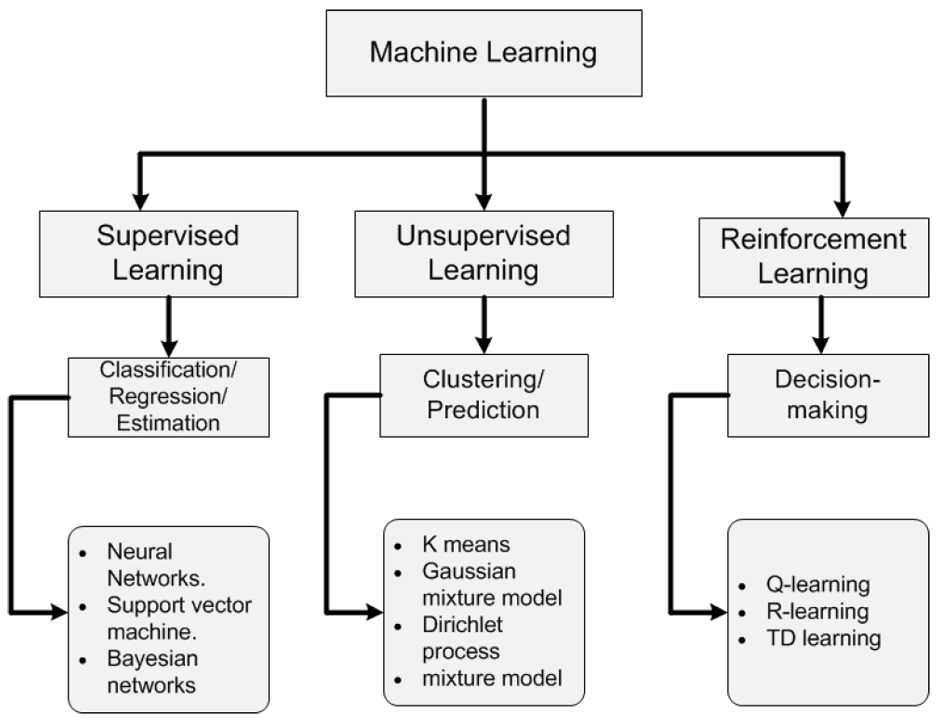
\includegraphics [scale=0.60] {my_folder/images/ch1/ML-categories.png}
	\caption{Категории ML и соответстующие алгоритмы. Основано на \cite{Sultan_2018}.} 
	\label{fig:ch1-ML-categories}
\end{figure}


\subsection{Обучение с учителем (Supervised Learning)}

\textbf{TODO: может быть добавить рисунок}

Один из способов машинного обучения, в ходе которого испытуемая система принудительно обучается с помощью примеров «стимул-реакция». С точки зрения кибернетики, является одним из видов кибернетического эксперимента. Между входами и эталонными выходами (стимул-реакция) может существовать некоторая зависимость, но она неизвестна. Известна только конечная совокупность прецедентов — пар «стимул-реакция», называемая обучающей выборкой. На основе этих данных требуется восстановить зависимость (построить модель отношений стимул-реакция, пригодных для прогнозирования), то есть построить алгоритм, способный для любого объекта выдать достаточно точный ответ \cite{james2014introduction}.

Обучение с учителем можно разделить на \textit{регрессию} и \textit{классификацию}, в зависимости от того, являются ли выходные переменные количественными или качественный. Количественные переменные принимают числовые значения, в то время как качественные переменные принимают значения в одном из K различных классов или категории \cite{james2014introduction}. Например, прогноз цены на жилье по данным параметрам, таким как местоположение дома, общая площадь и количество комнат и т. д., это проблема регрессии. Диагноз рака - проблема классификации поскольку выходной сигнал либо положительный, либо отрицательный.

В обучении с учителем набор данных делится на обучающий, набор для валидации и тестовый набор. Обучающий набор представляет собой пары ввода и вывода переменных, которые напрямую вводятся в модель для обучения. Валидационный набор используется для контроля за переобучением модели. Наконец, тестовый набор используется для подтверждения того, что обученная модель обобщена и точна

Обучение с учителем - наиболее распространенная категория в машинном обучении, но оно требует больших наборов данных с правильными «ответами». Это может быть очень дорого, в некоторых случаях не практично.


\subsection{Обучение без учителя (Unsupervised Learning)}
\textbf{TODO: может быть добавить рисунок}

Это ещё одна важная категория в машинном обучении.
В отличие от обучения с учителем, алгоритмы этой категории используют наборы данных, не размеченные «ответами». Задача в этой категории --- обнаружить скрытую структуру в данных и распределить их по группам.

Эта категория алгоритмов получила своё название из-за отсутствие меток или выходных переменных. Кластеризация является типичным инструментом, который используется чтобы понять связь между наблюдениями и распределить их в разные группы \cite{hastie2001elements}

При обучении без учителя данные не делятся на обучающие, проверочные и тестовые. Набор данных подается в модель напрямую и группируется в отдельные группы.


\subsection{Обучение с подкреплением (Reinforcement Learning)}

Последняя категория машинного обучения является междисциплинарной областью, которая сочетает в себе машинное обучение, неврологию, поведенческую психология, теорию управления и т. д. Цель RL заключается в достижении целей без четких инструкций, но с наградами или штрафами, получаемыми от взаимодействий с окружающей средой. 
% TODO: RL

Агент RL изучает оптимальную политику, последовательность действий, которая максимизируют общую будущую награду (Reward) \cite{SuttonAndBarto-RL-Introduction-p2}.

В обучении с подкреплением агент RL наблюдает состояние ${s_t}$ на этапе времени ${t}$, затем он взаимодействует с окружающей средой, выполняя действие ${a_t}$. Среда переходит в следующее состояние ${s_{t+1}}$, учитывая текущее состояние и выбранное действие, которое ведёт к получению агентом вознаграждения ${r_t}$. Цель агента узнать политику $\pi$, которая сопоставляет состояния с действиями, так что последовательность действий, выбранная агентом, максимизирует ожидаемое будущее вознаграждение. На каждом шаге взаимодействия со средой агент генерирует переход ${\{s_t, a_t, s_{t+1}, r_t\}}$, который даёт информацию, необходимую для улучшения политики, см. \firef{fig:ch1-RL-flow}.

\begin{figure}[ht!] 
	\center
	\includegraphics [scale=0.60] {my_folder/images/ch1/rl-flow.png}
	\caption{Агент взаимодействует с окружающей средой, сначала наблюдая состояние, затем совершая действие и, наконец, получая вознаграждения за выбранное действия. Через многочисленные попытки и ошибки, агент учится формулировать оптимальную политику \cite{SuttonAndBarto-RL-Introduction-p50}.} 
	\label{fig:ch1-RL-flow}
\end{figure}
% TODO: Перевести рисунок?
